\documentclass[12pt]{article}
\usepackage{amsmath,amssymb,bookmark,graphicx,parskip,wrapfig,custom}
\usepackage[margin=.8in]{geometry}
\allowdisplaybreaks
\hypersetup{colorlinks,
    citecolor=black,
    filecolor=black,
    linkcolor=black,
    urlcolor=black
}
\setcounter{secnumdepth}{5}

\begin{document}

\title{SCI 238 --- Introduction to Astronomy}
\author{Kevin James, Eric Pemberton, Lara Janecka, Nik Klassen, Tyler Babaran}
\date{\vspace{-2ex}Winter 2015}
\maketitle\HRule

\tableofcontents
\newpage


\input{chapters/chapter1.tex}
\input{chapters/chapter2.tex}
\input{chapters/chapter3.tex}
\input{chapters/chapter4.tex}
\input{chapters/chapter5.tex}
\input{chapters/chapter6.tex}
\section{Chapter 10 -- Our Star}
\subsection{A Closer Look at the Sun}
\subsubsection{History}
Our first views of the sun were that it was a ball of fire. In the $19^{th}$ century we had found the Sun's radius and distance and found that its energy could not have come from burning fuels or other chemical processes.

The first real idea was that the Sun generates energy by slowly contracting in size through \textbf{gravitational contraction}. Gravitational potential energy is converted into thermal energy as mass moves inward. This would keep the inside of the Sun hot. The amount of contraction required would be small enough to go unnoticed until the $19^{th}$ century. This theory shows that the Sun could continue contracting for 25 million years. The problem: geologists had already calculated the earth's age as much higher than that.

The next idea was based on Einstien's theory of relativity ($E=mc^2$). Calculations showed that the Sun had enough mass to shine for billions of years. This explained where sunlight came from, but not the thermal energy. Eventually in the  1930's the discovery of nuclear fusion was found and we use that to explain where thermal energy comes from.

\subsubsection{Nuclear Fusion}
Nuclear fusion requires very high temperature and density to start. This started in the sun through gravitational contraction. The sun was formed from a collapsing gas cloud. This released gravitational potential energy raisin the core temperature. This continued to happen until sustained nuclear fusion started.

The sun has a fairly steady size and energy today because it has reached equilibrium. \textbf{Gravitaitonal Equilibrium} is the balance between the outward push of hot internal gases trying to escape and the inward push of gravity. This allows the sun to have a steady size. This also means that \textbf{pressure increases with depth} in the sun. \textbf{Energy Balance} is the balance between the rate of fusion and the rate of energy being released from the Sun's core into space.

\subsubsection{Structure}
The sun is essentially a ball of plasma (gas in which atoms are ionized) which moves like a gas, but also reacts to magnetic fields.

Basic Properties:\\
\begin{tabular}{|c|c|}
\hline
Radius (R Sun ) & 696,000 km (about 109 times the radius of Earth)\\
\hline
Mass (M Sun )  & 2 ϫ 10 30 kg (about 300,000 times the mass of Earth)\\
\hline
Luminosity/Power Output (L Sun ) & 3.8 ϫ 10 26 watts\\
\hline
Composition (by percentage of mass) & 70\% hydrogen, 28\% helium,2\% heavier elements\\
\hline
Rotation rate & 25 days (equator) to 30 days (poles)\\
\hline
Surface temperature & 5800 K (average); 4000 K(sunspots)\\
\hline
Core temperature & 15 million K\\
\hline
\end{tabular}

Layers (outside in):
\begin{itemize}
\item Solar wind
\item Corona
\item Chromosphere
\item Photosphere
\item Convection zone
\item Radiation zone
\item Core
\end{itemize}
\textbf{Solar Winds} is a stream of charged particles blown outward from the Sun. These help shape the magnetospheres of planets and the tails of comets.

\textbf{Corona} is suprisingly hot (1 million K) and emits the most X-ray radiation, the density is very low

\textbf{Chromosphere} is much cooler here (10,000 K), radiates UV radiation

\textbf{Photosphere} temperature is 6,000K, surface churns like boiling water, home of sunspots and intense magnetic fields

\textbf{Convection Zone} region of hot gas rising and cool gas sinking caused by energy from the core rising to the surface (called convection, duh)

\textbf{Radiation Zone} less turbulent than the convection zone, energy moves outwards as photons instead of hot gas, temperature rises to 10 million K, shit ton of X-ray radiation

\textbf{Core} where nuclear fusion is making energy, temperature 15 million K, density 100 that of water, pressure 200 billion times earth's surface, energy takes hundreds of thousands of years to get to the surface

\subsection{Nuclear Fusion in the Sun}
Note nuclear fusion (the Sun) $\not =$ nuclear fision (nuclear reactor).

Within the Sun's core there is a soup of hot fas funn of psitively charged atom nuclei flying about. When these collide (most of the time electormagnetic forces deflect them) they stick together to form a heavier nucleus. This is caused by \textbf{strong force} (binds protons and neutrons together) overriding the electromagnetic deflection force. It's only strong enough to do this at very small distances which happens due to the high speed of the particles (which is in turn caused by the high temperature which is caused by the high pressure which is caused by high gravitational force which is caused by large mass).

This is explained by the \textbf{Ideal Gas Law} \[ P = nkT \] where P is the pressure, n is number density (particles per volume), T is temperature, and k is \textbf{Boltzmann constant} $=1.38 \times 10^{-23}$ joule/K

\subsubsection{Proton-Proton Chain}
Most hydrogen comes in the form of a single proton, but we need to fuse it into a helium atom which is two protons and two neutrons. So what we have to do is fuse four hydrogen atoms into one helium atom. This is through a sequence of events called the \textbf{proton-proton chain}.
\begin{enumerate}
\item Two protons fuse to make a deuterium nucleus (1 proton and 1 neutron). This step occurs twice
\item The deuterium nucleus and a proton fuse to make a nucleus of helium-3 (2 protons, 1 neutron). This step occurs twice
\item Two helium-3 nuclei fuse to form helium-4 (2 protons, 2 neutrons), releasing two excess protons in the process.
\end{enumerate}
In total four protons collide to make a helium atom, two positrons, and two neutrinos.

\subsubsection{Solar Thermostat}
Life on earth relies on the Sun's steady fusion rate. If we were to increase the core's temperature slightly, this would cause an increase in fusion rate. The increased fusion rate would make more energy, but energy moves very slowly through the sun so it would get bottled up in the core. This would increase the core pressure to exceed the balancing force of gravity so the core would expand and cool. Cooling lowers the fusion rate and equilibrium is reached again.

\includegraphics[width=\textwidth]{solarThermostat}

\subsubsection{Path of Energy Through the Sun}
Energy starts as photons in the Sun's core. They zigzag at the speed of light so it takes them a while to get out. In the dense interior a photon can only ravel a fraction of a millimeter before it collides with electron and gets deflected in a new direction causing its zigzag path. Eventually it makes its way through the core and radiation zone into the convection zone where the temperature drops to 2 million K and the photon is absorved into cooler solar plasma. This creates the convection that happens in the convection zone. Eventually it rises to the top and enters the photosphere. Here the density is low enough that photons can escape into space as sunlight.

How do we know about the interior of a star:
\begin{itemize}
\item Mathematical models: based on laws of physics and observed properties
\item Solar Vibrations: the Sun's surface vibrates like with earthquakes which we can see in Doppler Shifts.
\item Solar Neutrinos: these are formed during nuclear fusion, these can pass through almost anything without reacting (including the Sun's layers), so we can see whats going on right now (well, 8 minutes ago)
\begin{itemize}
\item these fuckers are hard to catch, need detectors deep in mines
\item initially we only caught a third of what we expected (solar neutrino problem) due to neutrinos changing properties during their journey (electron neutrino, muon neutrino, or tau neutrino)
\end{itemize}
\end{itemize}

\subsection{The Sun-Earth Connection}
\subsubsection{Sunspots and Magnetic Fields}
\textbf{Sunspots} are dark spots on the sun where things are cooler. They are formed when magnetic fields keep hot gas from entering a section of the photosphere. Magnetic fields can alter the energy levels of atoms (Zeeman effect), mucking with their spectral lines. The particles in solar plasma move along magnetic lines (usually spiraling along them).

Sunspots form where magnetic fields extend from the Sun's interior. The magnetic lines there are strong enough to suppress convection making the spot cool. They usually last a few weeks until their magnetic fields weaken. Sunspots tend to appear in pairs connected by a magnetic loop. Gas getting trapped in these loops makes \textbf{solar prominences}.

\subsubsection{Solar Storms}
These are sudden changes in the Sun's magnetic fields. The most dramatic example is \textbf{solar flares} which send bursts of X rays and fast moving particles into space. Flares tend to happen near sunspots. The current theory is that solar flares are caused when magnetic fields become so twisted they cannot bear the tension and snap into a better shape.

\subsubsection{Heating the Chromosphere and Corona}
Some weird shit goes down on the sun where its atmosphere gets hotter the farther you go out. The current theory is that magnetic fields carry energy upward to heat the chromosphere and corona.

The churning that happens in the convection zone probably shakes with tightly wound magnetic lines which carry this energy into the atmosphere and deposit it as heat.

Its very hard to investigate this because the solar atmosphere is not dense enough to see at that point (except during an eclipse). We can watch them through X-rays and UV rays.

In X-ray images of the chronosphere:
\begin{itemize}
\item bright spots is where hot gas is trapped below a sunspot where magnetic lines loop back to the Sun
\item dull spots (\textbf{coronal holes}) are under magnetic lines that escape into space
\item the stuff blown out by flares are huge bubbles called \textbf{coronal mass ejections}
\begin{itemize}
\item have strong magnetic fields
\item causes auroras
\item fuck with satellites
\end{itemize}
\end{itemize}

\subsubsection{Solar Cycles}
Sunspots have a 11 year cycle. The solar maximum has most sunspots and solar minimum has fewest. At each solar maximum the Sun's magnetic fields start to flip. This is because all magnetic lines connecting pairs of sunspots point the same direction. This means that magnetic fields have a 22 year cycle.

\section{Chapter 11 -- Surveying the Stars}
\subsection{Properties of Stars}
\subsubsection{Luminosity}
The \textbf{apparent brightness} of a star is how bright it appears to us, or the amount of power reaching us per unit area (units are watts per square meter). The \textbf{luminosity} of a start is is the total power that the star emits (units are watts). Apparent brightness follows a inverse square law to distance.
\begin{align*}
    \text{apparent brightness} = \frac{\text{luminosity}}{4\pi \times (\text{distance})^2}
\end{align*}

The most direct way to measure a star's distance it through measuring its stellar paralax. This is found by comparing a star's shift against its background over 6 months. We calculate its \textbf{paralax angle} \[ d = \frac{1}{p} \]
Where d is the distance to that star in light years and p is the paralax angle (Note: 1 arcsecond $\rightarrow$ 3.26 lightyears = 1 parsec)

We tend to measure luminosities as orders of magnitude of our sun's luminosity, called \textbf{apparent magnitude} instead of apparent brightness and \textbf{absolute magnitude} instead of luminosity. For every 5 magnitudes we have a brightness factor of 100. So a magnitude 1 star is 100 times brighter than a magnitude 6 star. We define the absolute magnitude as the apparent magnitude if owould have itf it were at a distance of 10 parsecs.

\subsubsection{Temperature}
The temperature of a star usually means its surface temperature since its the easiest to measure. A star's temperature is easier to measure than luminosity since it does not vary with distance. We can measure a star's temperature with reasonable accuracy by measuring its color. This is done by comparing its apparent brightness in two different colors of light (usually blue and red).

We run into problems when interstellar dust interferes with the color of a star so astronomers use a star's spectral lines instead. Stars showing spectral lines of ionized elements are fairly hot because it takes high temperature to ionize atoms. In contrast, stars displying spectral lines of molecules are relatively cool. Stars are classified by their \textbf{spectral type} OBAFGK in decreasing order of temperature. These are often divided farther using numbers. For example our sun is a G2 star meaning its hotter than a G3 but cooler than a G1.

\begin{tabular}{|l|l|l|l|l|}
\hline
Type & Example(s) & Temp. & Key Absorption Line Features & Brightest (color) \\
\hline
O & Stars of Orion’s Belt & $>$30k K & Strong ionized He, weak H & $>$97 nm (ultraviolet) \\
\hline
B & Rigel & 30k-10k K & Strong neutral He, some H & 97-290 nm (ultraviolet) \\
\hline
A & Sirius & 10k-7.5k K & Very strong H & 290-390 nm (violet) \\
\hline
F & Polaris & 7.5k-6k K & Some H, some ionized Ca & 390-480 nm (blue) \\
\hline
G & Sun, Alpha Cent. A & 6k-5k K & Weak H, strong ionized Ca & 480-580 nm(yellow) \\
\hline
K & Arcturus & 5k-3.5k K & some metals, some molecules & 580-830 nm (red) \\
\hline
M & Betelgeuse, Prox. Cent. & $<$3.5k K & Strong molecules & $>$ 830 nm (infrared) \\
\hline
\end{tabular}

\textbf{History of Spectral Types}
Spectral types were made at Harvard College by Edward Pickering's computers (women who'd studied physics or astronomy). The first was Williamina Flemming who classified A-O by the descending strength of hydrogen lines. Annie Jump Cannon modified this existing classification by reordering and removing classes until the OBAFGKM that is used today was left. Finally Cecilia Payne-Gaposchkin discovered that stars were all made of the same material and the lines reflected ionization levels which indicated surface temperature.

\subsection{Mass}
Measuring mass is very difficult and we can only really do it on binary star systems. We do this by applying Newton's version of Kepler's third law

Binary star types:
\begin{itemize}
\item \textbf{visual binary: } we can see each star distinctly, sometimes one star is too dim to see but we can observe the shift of the visible star
\item \textbf{eclipsing: }  a pair of stars that orbit in a plain of our line of sight, we rotate between seeing the combined light of both stars (no eclipse) and only the light of one star (full eclipse)
\item \textbf{spectroscopic: } we need to use Doppler shifts to detect its nature
\end{itemize}

\subsection{Patterns Among Stars}
These are ways of charting stars, the x-axis is the surface temperature (OBAFGKM) and the vertical axis is luminosity ($L_{sun}$) on a logarithmic scale. We can also infer the star's radius from the chart because a star's luminosity is based on its surface temperature and radius.
\begin{align*}
L &= 4\pi r^2 \times \sigma T^4 \\
\sigma &= 5.7 \times 10^{-8} W/(m^2 \times \text{Kelvin}^4)
\end{align*}
Where L is luminosity, r is radius, $\sigma$ is amount of thermal radiation emmited per unit area constant, and T is the star's temperature. This means that the radius of a star increases along a diagonal from lower left to upper right.

Stars cluster on the H-R diagram:
\begin{itemize}
\item \textbf{main sequence: }streak running from upper left to lower right
\item \textbf{supergiants: }upper right
\item \textbf{giants: }between supergiants and main sequence
\item \textbf{white dwarfs: }lower left
\end{itemize}

Like with spectral classes, astronomers assign luminosity classes describing the region of the H-R diagram that a star falls in. I is for super giants, III is for giants and V is for main sequence. II and IV are for those that fall inbetween. White dwarfs fall outside the classification and are called wd. Stars with higher luminosity have larger radii as well.

We combine spectral type and luminosity class together to identify stars.

\subsection{Main Sequence}
Main sequence stars are the majority of stars that we observe and because of that we have found more patterns within them. Mass increases as we go up the strip of main sequence stars on the H-R Diagram. We also see that low mass stars are much more common than high mass stars. Mass is the most important attribute of hydrogen fusing stars because it determines the balance point at which energy released by fusion equals the energy lost from the star's surface. This is what allows for the wide range of luminosities. Luminosity is very sensitive to mass (example a star 10 times as massive as the sun is 10000 times as luminous).

A luminous star must be very hot or very large. But a very small mass change is required to greatly increase the luminosity of a star, so their surface temperature must be much higher to account for this large increase in luminosity. This fits the H-R Diagram pattern of temperature increasing with luminosity. We can use the mass-luminosity-temperature relationship to estimate a star's mass just by knowing its spectral type.

A star is born with a set amount of hydrogen fuel, the amount of time that it can burn this fuel for is the star's \textbf{main sequence lifetime}. Lifetime is inversely proportional to the mass of the star. This is because as mass increases luminosity increases exponentially, so stars with higher masses may have more fuel but they burn it waaaay faster.

\subsection{Giants, Supergiants, and White Dwarfs}
\subsubsection{Giants and Supergiants}
These are much cooler but more luminous than the sun which tells us that they are huge. These stars have almost exhausted their hydrogen fuel supply and are trying not to collapse under their own weight. They do this by releasing fusion energy at a high rate which explains their high luminosity, and the need to radiate all this energy expands them to enormous size.

\subsubsection{White Dwarfs}
This is what happens when a giant runs out of fuel completely. The star ejects all of its outer layers and is left only with a dormant core. They are hot because they are still the core of a star, but dim because they have no way to radiate their energy.

\subsection{Star Clusters}
Stars are born from giant clouds and many stars can be born from the same cloud, so they tend to cluster.
\begin{itemize}
\item all stars in a cluster are about the same distance from earth
\item all stars in a cluster are about the same age
\end{itemize}

\subsubsection{Types of clusters}
\begin{itemize}
\item \textbf{open cluster: }found in disk of galaxy, young stars, up to several thousand stars, about 30 light years across
\item \textbf{globular cluster: }found in halo of galaxy: oldest stars, more than a million stars, 60-150 light years across
\end{itemize}

\subsubsection{Age of a Cluster}
We plot a cluster's stars on the H-R Diagram, and this tells us its age. For instance the Pleides open cluster has no stars of the O spectral class. This means that Pleidas is old enough that its O stars have finished their hydrogen fission and `died'. We call the point at which a cluster's main sequence diverges from the standard main sequence the \textbf{main sequence turnoff}. The age of the cluster is equal to the lifetime of stars at its main-sequence turnoff point (at its most massive star).

\section{Chapter 12 -- Star Life Cycle}
All elements heavier than hydrogen and helium were created through fusion or supernova

\subsection{Star Birth}
gravity causes a gas cloud to contract until center is hot enough to sustain -fusion
heat generated from gravitational potential
clouds internal gas pressure resists gravity

gravitational equilibrium: gas pulling inward matches pressure pushing out, star size is stable

two factors:
    1. higher density, more material per space (still low enough to be strong vacuum on earth)
    2. lower temperature, reduces pressure (typically 10-30 K)

$M_min = 18 * M_Sun * sqrt(T^3 / n)$

T = temp of gas in K
n = density of gas in particles per cubic meter

referred to as molecular clouds, cold enough for H atoms to pair up
very large, many stars generally born in simulatneous clusters


\subsubsection{Protostar Stage}
    as it compresses gas starts to heat up, lumpy clumpy shape
    energy radiates away until its dense enough to trap heat, temp rises hard
    still not hot enough for fusion
    rotate rapidly from conservation of momentum of particles
    flattens to a disk from particle collisions (plantes may form here eventually)
    may shoot jets perpindicular to disk (not sure why, suspect magnetic fields due to rotation)
    field also generates protostellar wind (stronger version of solar wind)
    wind and jets shed momentum by expelling material, slowing rotation

    angular momentum also cause of binary star systems (stars form close together, orbit instead of crash, more momentum = larger orbit)

    becomes true star at 10 million K, continues to rise until balance achieved (energy from fusion = energy radiated)
    time to reach main sequence phase proportional to mass, large stars are faster

stars range in size, over 99\% are within 0.5 and 2 M\_Sun (leaning below 1)
large ones burn out faster

stars cant be more than 300 M\_Sun because it would blow off its outer layers
cant be less than 0.08 M\_Sun or it wont get hot enough, stabilizes as a brown dwarf
brown dwarf gravity collapse halted due to degeneracy pressure, restriction on how close elections can be together

\subsection{Low Mass Stars ($<8$ M\_sun)}
    Main-Sequence stage
        90\% of star's lifetime
        star regulates itself: if fusion works too fast, core expands until it cools again

    \subsubsection{Red Giant stage}
        when core hydrogen is depleted, fusion will cease
        no more radiation pushing outwards, core shrinks from gravity
        core is inert helium, small shell of hydrogen around it fuses (higher rate than core), outer layers expand
        star is 100 times larger and 1000 times brighter than main sequence stage
        weaker gravity at surface, increased stellar wind
        fusion shell makes more helium, core gets heavier and shrinks more, shell gets even hotter and denser

    \subsubsection{Helium Core Fusion stage}
        feedback loop until core reaches 100 million K, helium start fusing into carbon
        at this point thermal pressure is too low (gravity is fucking intense)
        core sustained by degeneracy pressure, which does not increase with temperature
        helium fusion heats the core without causing it to inflate, fusion rate spikes (called helium flash)
        so much so that thermal pressure becomes dominant and core increases in size, lowering temp and fusion
        outer layers shrink again, stabilizes back at yellow
        this stage is short, 1\% of star lifetime

    \subsubsection{Last Gasps}
        when helium runs out carbon core shrinks again
        outer layer expansion again from helium shell fusion (hydrogen shell still going, core double layered)
        now even larger than red giant stage
        star is too low mass to fuse carbon, will not reach 600 million K
        too large  for its mass, gravity too low on surface, outer layers start being blown off
        forms planetary nebula (nothing to do with planets), bright glowing ring
        will combine into interstellar dust when cooled
        exposed core remains as a stable white dwarf, gas recycled into a new star
        will cool until it no longer emits light, then sit in the dark of space


\subsection{High Mass Stars}
    \subsubsection{Hydrogen Fusion}
        once in main stage, protons can slam into carbon, nitrogen, oxygen molecules with enough energy
        follows CNO cycle of fusion and decay
            1. C12 + H -> N13
            2. N13 -> C13
            3. C13 + H -> N14
            4. N14 + H -> O15
            5. O15 -> N15
            6. N15 + H -> C12 + He4

        this cycle allows hydrogen fusion to proceed much faster than proceed much faster than typical proton chain (more valid things to bump into)
        makes these stars much brighter, lives much shorter

    \subsubsection{Becoming a Supergiant}
        reaches hydrogen fusing shell stage much faster, outerlayers expand
        temperatures so high that degeneracy pressure never takes over, no helium flash (gradual, like hydrogen was)
        fuses helium into inert carbon core in just a few thousand years
        core fusion stops, core shrinks, helium shell forms, surface expands
        alternates between shrinking and expanding as core reaches next level of fusion
        hydrogen > helium > carbon > oxygen > neon > magnesium > silicon > iron
        the biggest stars transitions so quickly other layers dont have time to resond, become red supergiant

        eg Betelgeuese, Orion's left shoulder. 500 solar radii, 2 AU

    \subsubsection{Heavier Nuclei}
        simplest heavy fusion is helium-capture reaction
            1. C12 + He4 -> O16
            2. O16 + He4 -> Ne20
            3. Ne20 + He4 -> Mg24

        note that each transition upwards drains the core and causes another shell to form
        all shells will be active simultaneously
        once hot enough, can start fusing those heavy nuclei
            1. C12 + O16 -> Si28
            2. O16 + O16 -> Si31 + H
            3. Si28 + Si28 -> Fe56

    \subsubsection{Iron, the Dead End}
        iron is the only element where it is not possible to generate nuclear energy, fusion or fission
        lowest mass per nuclear particle of all elements
        iron core can only resist gravity through degeneracy pressure, but more iron keeps piling on
        then gravity pushes past the quantum mechanical limit

    \subsubsection{Supernova}
        electrons disappear by combining with protons to form neutrons, realeasing neutrinos
        iron core with a mass near M\_Sun and radius larger than Earth collapses into a ball of neutrons just a few kilometers across in a fraction of a second
        stops due to neuton denegeneracy pressure
        this neutron star is similar to an atom nuecleus the size of Kitchener
        the gravitational collapse of the core releases an enormous amount of energy, more than 100 times than the Sun will radiate over its entire 10 billion year lifetime
        old theory was that supernova was caused by matter collapsing into neutron star and bouncing
        new theory is collapse causes so many neutrinos to be formed that, despite how rarely they interact with matter, entire star is blown away
        so hot that it's as bright as moderately sized galaxies for a few weeks, continue to expand and cool
        will eventually be incorporated into new stars in other gas clouds

    Crab nebula is remnant of supernova from 1054 AD

    if gravity is still strong enough to overcome neutron degeneracy pressure, collapses continues further to a black hole

    interesting note: due to larger stars dying and adding heavier elementss to the interstellar dust, newer stars have higher percentages of heavy elements than older stars (2-3\% vs 0.1\%)

    interesting note: most heavy elements are made in helium capture which adds two protons, so even numbered elements are more abundant in the universe


\subsection{Binary Systems}
    the two stars exert tidal forces on eachother, create football shapes
    when the more massive star begins to expand, the gas on the surface experiences strong pull to the other star than its own core, begins a mass exchange
    may transfer back when "soon to be as or more massive" star begins expanding too

\section{Chapter 13 -- White Dwarfs, Neutron Stars, Black Holes}
To scientists, dead stars are ideal laboratories for testing the most extreme theories of general relativity and quantum theory.

\subsection{White Dwarfs}
\subsubsection{What is a white dwarf?}
A white dwarf is essentially the exposed core of a low-mass star that has died and shed its outer layers in a planetary nebula. It is quite hot when it first forms (it was the inside of a star) but it slowly cools with time. White Dwarfs have masses like those of stars but sizes like that of Earth which is why they are generally quite dim compared to stars like the sun. THe hottest white dwarfs can shine brightly in high-energy light such as ultraviolet and X-rays.

A white dwarf's combination of starlike mass and a small size makes gravity near its surface very strong. Because there is no fusion to maintain heat and pressure, {\bf degeneracy pressure} combats the gravitational force. The same pressure supports brown dwarfs, it arises when particles are packed as closely as the laws of quantum mechanics allow. More specifically, in white dwarfs arises from electrons so it is called {\bf electron degneracy pressure}

\subsubsection{Composition, Density and Size}
{\bf Composition} of a White Dwarf reflects product's of stars final fusion stage. A white dwarf from something resembling our sun would consist mostly of carbon. (stars like the sun fuses helium into carbon in final stage of life). The {\bf bf denisty} of a white dwarf is so high that a teaspoon of its material would weight several tons. More massive white dwarfs are also smaller in size (the most massive being the smallest). The more massive a white dwarf is, the greater gravity compresses matter to a much greater density. Electrons in a white dwarf respond to compression by moving faster.

\subsubsection{The White Dwarf Limit}
The fact that electron speeds are higher in more massive white dwarfs leads to a fundamental limit on the maximum mass of a white dwarf. The {\bf White Dwarf limit} is {\bf $1.4M_Sun$} because anything larger than this would have electrons moving faster than the speed of light. Also called Chandrasekhar limit. In every observed case this limit holds true.

\subsubsection{White Dwarf in a binary System}
A white dwarf in a binary system can slowly gain mass if its companion is a main sequence of giant star. Matter coming from the other star forms a whirlpool like disk as it makes its way to the White Dwarf's surface (called an {\bf accretion disk}). In this way, a white dwarf can get Hydrogen.

{\bf Novae}: Hydrogen spilling towards the white dwarf heats up. If the temperature reaches 10 million K hydrogen fusion suddenly ignites. This thermonuclear flash causes the binary system to shine for a few weeks as a nova. (far less luminous than a supernova but can still shine as brightly as 100,000 suns). Accretion resumes after nova explosion subsides so process can repeat itself

{\bf White Dwarf SuperNovae}: Through repeating the previous process it is believed that a white dwarf gains mass. When it reaches the {\bf white dwarf limit} carbon fusion begins and explodes completely into what we call a {\bf White Dwarf Supernova}. This is however quite different from a {\bf massive star supernova}. Both shine with luminosities of 10 billion times that of the Sun but white dwarfs supernovas fade steadily and massive stars are more complicated. White Dwarf supernovas also lack hydrogen lines.

\subsection{Neutron Stars}
\subsubsection{What is a neutron star?}
A ball of neutrons created by the collapse of the iron core in a massive star supernova. Typically 10km in radius yet more massive than the sun. {\bf Neutron degeneracy pressure} supports neutron stars. The gravity on the surface makes the escape velocity about half the speed of light. Neutron stars spin rapidly when they are born and strong magnetic fields can direct beams of radiation that sweep through space.

\subsubsection{How were they discovered?}
First observational evidence 1967, radio waves at precise intervals (now refered to as {\bf pulsars}). Signal came from gaseous remains of supernova. It was a neutron star, pulsations arise becuase of conservation of angular momentum (rotation increases as size decreases). Neutron star's rotation slows over time. {\bf Pulsars} must be neutron stars because no other object could spine that quickly without tearing itself apart. White Dwarf 1/sec. Pulsar as fast as 625/second.

\subsubsection{Neutron Star in a binary System}
Like white dwarfs, neutron stars can burst back to life. Due to stronger gravity, the accretion disk on a neutron star is much hotter and denser than a white dwarf's. High temperatures in inner regions of the disk make it radiate powerfully in x-rays. Due to this emission these are often called {\bf X-ray binaries} and hundreds have been detected in the Milky Way. Pulsars of X-ray binaries accelerate with time, some rotating every few thousandths of a second. (called {\bf millisecond pulsars}).

Helium fusion can happen at a layer of the disk builds to 100 million K. Helium fuses rapidly and generates an {\bf X-ray burster} which lasts a few seconds and flares every few hours to every few days. Energy relased is 100,000 times more powerful than sun output, all in X-rays. After burst, accretion resumes.

\subsection{Black Holes}
\subsubsection{What is a Black Hole?}
A black hole is so compact that it has an escape velocity greater than the speed of light, neither light nor anything else can escape from within a black hole. They are actually spherical and not funnel shaped.

{\bf The Event Horizon}: The boundary between the inside of a black hole and the universe outside is called the event horizon. It marks the point of no return for objects, the boundary at which escape velocity equals the speed of light. Gets the name because we have no hope of learning about events that occur within it.

The {\bf size} of a black hole is usually the size of its event horizon, defined by the {\bf Schwarzschild radius}. Black hole with mass of the Sun has a Schwarzschild radius of about 3km. More massive black holes have a larger Schwarzschild radius.

A collapsing stellar core becomes a black hole at the moment it shrinks to a size smaller than its Schwarzschild radius.

Schwarzschild radius: \[ R_s = \frac{2GM}{c^2} \]

\subsubsection{Singularity and Limits of Knowledge}
Because nothing can stop the crush of gravity in a black hole, we might expect all matter that forms a black hole must ultimately be crushed to an infinitely tiny area and dense point in the center called a {\bf singularity}

According to Einstein's theory from your point of view a friend would never cross the event horizon even though he would vanish from view due to redshifiting. You would not survive to cross the event horizon due to gravity, however with supermassive black holes, tidal forces are weaker so it would be possible to enter the event horizon.

\subsubsection{Formation of a Black Hole}

Most massive stars may not succeed in blowing away all upper layers in supernova. If enough mass falls back to neutron star, it could exceed neutron star limit (3M Sun). Gravity would exceed degeneracy pressure and core collapses again with no known force to keep it from collapsing into a black hole.

\subsubsection{Observational Evidence}
Gravity alters its surroundings. Compelling observational evidence comes from studying X-ray binaries, some may contain black holes instead of neutron stars. The trick to learn is by measuring mass.

\subsection{Origin of Gamma Ray Bursts}
By far the most powerful bursts of energy we observe in the universe. Some appear to come from extremely powerful supernova explosions. A supernova from a neutron star does not release enough energy, however a supernova that forms a black hole ({\bf hypernova}) might be powerful enough to explain it.

\subsection{Summary Notes}
\begin{itemize}
\item Observation evidence exists for white dwarfs and neutron stars, is strong for black holes
\item All three can have close stellar companions in which they can accrete matter.
\item Black holes are holes in the universe that strongly warp time and space around them. Nature of singularities beyond frontier of current understanding.
\end{itemize}

\input{chapters/chapter14.tex}
\input{chapters/chapter15.tex}
\section{Chapter 16 -- Dark Matter, Dark Energy, and the Fate of the Universe}
The dominant source of gravity in the universe is {\bf dark matter}, which is completely unobservable. {\bf Dark energy} seems to be counteracting the effects of gravity on a massive scale.

In fact, the universe itself seems to be mostly composed of dark matter, rather than of atoms. Basically, dark matter is a theorized bunch of matter than may or may not exist but is necessary to create the effects our models predict. It is matter that gives off no light, ie. remains ``dark''.

We predict that the expansion of the universe must slow over time due to the diminishing effects of gravity. If it does not, there must exist some ``dark'' energy fueling the expansion. Note that sometimes we refer to dark energy as {\bf quintessence} or a {\bf cosmological constant}. There is also no real correlation between dark matter and dark energy, other than that we have determined their existance through their being {\it necessary}.

\subsection{Evidence}
We know that distance from the center of a circle and an object's orbital relation are related. It turns out if the center of the circle is the center of mass, the orbital speed {\it decreases} as we move away from the center. If the mass is distributed evenly, the orbital speed {\it increases}. Since the orbital speed of the stars within our galaxy increase as we move away from the galactic center, there must be a large amount of mass on the galaxy's halo. Since we can detect no radiation from it, we call that dark matter.

For galaxies that are not our own, we can make a similar calulation: using the mass-to-luminosty ratio, we can determine the total mass of the galaxy. Then, we can measure the velocities of stars and dust clouds in that galaxy and use the laws of galaxy to caluclate their mass. The difference in mass is dark matter.

We find that the composition of a spiral galaxy is typically 98\% or more dark matter.

We can apply these same techniques to galactic clusters. If we assume they orbit each other, the gravitational calculations predict a far greater mass than their luminosities would. Thus we see that Galactic clusters are even more than 90\% percent dark matter!

We can also measure the temperature of the hot gas (interstellar medium) within a galaxy by measuring the X-rays that medium emits. Since temperature is related to mass in this case, we can determine a galaxy's total mass with some calculations. Studies performed using this method see galaxies as containing more mass than luminosity would predict and thus agree with the above gravitational calculations.

We can also use {\bf gravitational lensing} to make the mass measurements. This technique relies on large masses ``bending'' light as it travels by exerting gravitational influences on the photons. By measuring the perceived shift, we can determine the mass of the objects between us and a source of light. By using this technique, we can use Einstein's Laws instead of Newton's. Since these results agree, we can increase our confidence in dark matter.

We are pretty sure that there are two options:
\begin{itemize}
\item our understanding of gravity is correct and dark matter exists, or
\item our understanding of gravity is incorrect.
\end{itemize}

That said, we are quite confident in our understanding of gravity. Furthermore, no one has been able to come up with an explanation which neatly explains our observations.

\subsection{Composition}
Dark matter may either be composed of particles we have already detected -- but in some form as to be undetectable -- or of exotic particles. At least most of it is likely exotic.

Dark matter could contain some non-exotic matter: if your body were in space, it would be undetectable as it would not be luminous enough to be visible. Similarly, planets, brown dwarfs, faint red M-sequence stars, etc are also classified as dark matter since they are too dim to be seen. That siad, if dark matter contained any of these objects, we could detect it: due to gravitational lensing, any of these objects passing in front of any source of light would be noticeable. The duration of this lensing would reveal the object's mass. We have discovered a few of these events, but not nearly enough to explain dark matter's prevalance or mass. Similar measurements agree dark matter can not be mostly comprised of black holes.

Models of nuclear fusion give us an estimate of the total number of protons, neutrons, etc in the galaxy. Their mass would comprise about one-sixth of the measured mass of the universe; thus there must be some exotic particles filling the five-sixths of the universe's mass.

We imagine dark matter to be composed heavily of {\bf weakly interacting massive particles}, or {\bf WIMPs}. These particles would be similar to neutrinos, in that they interact only with a couple of the four forces (ie. weakly interact) but far more massive and slower moving. Note that though these are refered to ass ``massive particles'', they are really subparticles and are thus only massive relatively speaking.

A large amount of WIMPs being present in the outer halo of a galaxy fits within our current understanding.

We have not yet detected any WIMPs, but through large-scale space particle detection and particle colliders, we are hopeful we will detect some soon.

\subsection{Dark Matter's Role}
Dark matter likely played an essential role in formating galaxies: by being os large in mass, areas high in dark matter likely attracted many other particles and eventually developed the mass to become a galaxy.

We also know that the universe is arranged into galactic clusters, superclusters, and even large sheets of superclusters. The reason mass in our universe is so highly divided is likely due to the effects of gravity from large amounts of dark matter. In fact, the current galactic structure likely mirrors the initial distribution of dark matter.

\subsection{The Fate of the Universe}
We can determine a {\bf critical density} of our universe by which a universe with a larger density will eventually start contracting and one with a smaller density will simply expand forever. Including dark matter, our estimates of the universe's matter content fall short of this critical density (we measure mass approximately equal to 0.5\% of the required amount and believe dark matter is 50 times more massive, thus we have 25\% of the required mass). Thus the universe seems likel to continue expanding forever, as we are doubtful there is more dark matter than we have predicted.

In fact, the expansion of the universe is {\it increasing} over time, which should not happen based on our understanding of gravity. Thus we label dark energy as the force causing the expansion.

\subsubsection{Expansion Patterns}
Given future changes in expansion rates, we determine four possible expansion patterns:
\begin{description}
\item[recolapsing] if there were no dark energy and the universe was above critical density, universal expansion would eventually reverse and end in a ``big crunch''. This is sometimes refered to as a {\bf closed universe}, since it could be modelled by a mathematically closed sphere in more dimensions.
\item[critical] if there were no dark energy and the universe was at critical density, the universe's expansion would slow over time but never reverse. Mathematicall, we could call this a {\bf flat universe}.
\item[coasting] if there were no dark energy and the universe was below critical density, the universe would keep expanding at its current rate forever. We could mathematically call this an {\bf open universe}.
\item[accelerating] if dark matter exerts a repulsive force which causes the universe's expansion to acclerate over time, the universal expansion rate would increase over time. This type of universe may be closed, open, or flat. Current evidence points to our universe being an accelerating flat universe.
\end{description}

Based on the average distance between galaxies over time, we seem to be in an accelerating universe. We measure this by looking at white dwarf supernovae: their distance tells us the lookback time and their redshift tells us what rate the galaxy had been expanding at.

\section{Chapter 17: The Beginning of Time}
\subsection{The Big Bang}
We can use light from distant galaxies to see about a billion years into the past, beyond this we cannot see any objects bright enough. We also run into a problem with background radiation left over from the Big Bang. This radiation is from when the universe was 380 000 years old (before that light could not pass through). Most of our knowledge of the Big Bang is from mathematical models.

\subsubsection{Conditions of the Early Universe}
During the first few seconds the universe was so hot that photons could transform themselves into matter and back. When two photons collide with energy twice that of a electron (its mass times $c^2$) they make a electron (matter) and positron (antimatter). When these two meet they annihilate each other and release photon energy. Similar actions can be done for protons and neutrons. At its start, the universe was full of matter and antimatter jumping to and from energy.

Forces:
\begin{itemize}
\item Gravity: holds planets together (dominant on large objects)
\item Electromagnetism: holds particles together (dominant on atoms and molecules)
\item Strong nuclear: holds atom nucleus together
\item Weak nuclear: deals with fusion and fission
\end{itemize}

At high temperatures (like at the birth of the universe) some of these meld into a different force. At its very start the universe was governed by one super force.

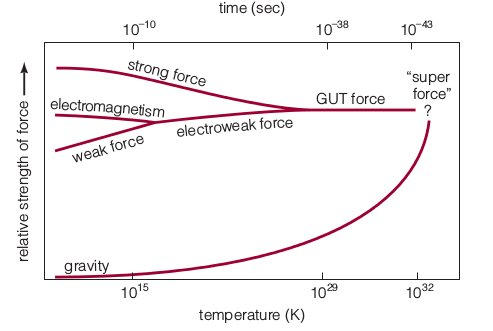
\includegraphics[scale=0.5]{forces}

\subsubsection{History of the Universe}
We break the history of the universe into eras.

\begin{wrapfigure}{l}{5.5cm}
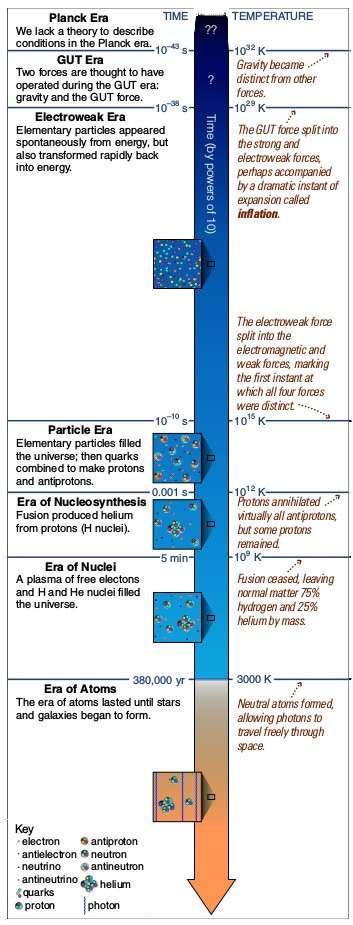
\includegraphics[width=5.5cm]{eras}
\end{wrapfigure}

\textbf{Planck Era}
This is the limit of what our current understanding of physics can explain. At this point we know that mass and energy were being converted back and forth rapidly. These energy fluctuations caused a changing gravitational field that warped space and time. A problem arises in that we have no theory to link quantum mechanics and general relativity. This era ended when the universe cooled enough for the super force to break into GUT force and gravity.

\textbf{GUT Era}
We know barely more about this era than we do about the Planck era, and even then what we know is not well tested. We think that the separation of GUT into strong and electroweak forces released a ton of energy causing a dramatic expansion of the universe called \textbf{inflation} (we think expanding things of atomic size to solar system sized).

\textbf{Electroweak Era}
At the end of this era the electroweak force breaks apart into the electromagentic and weak nuclear forces. This is the first point where we have experimental evidence of things actually fitting our models. Particle accelerators produced weak bosons that we predicted would exist during this era.

\textbf{Particle Era}
This is the era right before the crazy energy-particle switching calmed down. All of the quarks created during this era had combined into protons and neutrons by its end. Since we were not spontaneously making matter and antimatter the two started permanently annihilating each other. We know that matter out numbered antimatter because matter exists. By comparing estimates on how many protons and photons there are we can get a rough estimate of the size of matter antimatter imbalance. The two numbers would have been similar at the start of the universe, but now photons outnumber protons a billion to one. This means that for every billion antiprotons there were a billion and one protons so when the billion annihilated themselves they made a billion extra photons.

\textbf{Era of Nucleosynthesis}
Now that we had a steady amount of matter it started fusing into heavier elements but the heat of the universe kept breaking them apart. At the end of this era it had gotten too cool to fuse heavier elements.

\textbf{Era of Nucleus}
At this point the universe consisted of plasma made of hydrogen and helium nuclei and electrons. Light didnt really go anywhere because it just bounced around between electrons (like it does inside a star). At the end of this era the universe had cooled enough for the nuclei to snag electrons and become stable. Once that happened light could travel in straight lines.

\textbf{Era of Atoms and Era of Galaxies}
Now that we have stable atoms we can be in the era of atoms. The universe is now a mix of neutral atoms, plasma, and photons. Slight areas of higher density started attracting atoms and plasma to make protogalactic clouds. These went on to form stars and eventually galaxies. This is the era we are currently in.

\subsection{Evidence}
The big bang theory is widely accepted because it accurately predicts \textbf{cosmic background microwave radiation} as the radiation that started streaming through the universe at the end of the nuclei era. It also accurately predicts the amount of helium in the universe.

\subsubsection{Left Over Radiation}
Arno Penzias and Robert Wilson kept hearing noise on their microwave antenna, this was background radiation from the universes formation. They found that the noise was exactly the same from every direction (so it wasn't just coming from something). At the same time a group at Princton had found that the radiation created during the formation of the universe (predicted by George Gamow) would have to still exist and be detectable with microwave antennas.

Scientists predicted that cosmic background radiation would have a prefect thermal spectrum since it was from the start of the universe. Since it broke free when the universe was the temperature of a red giant it should have the same signature, but stretched by 1000 (since thats how much the universe has expanded since then). This shifted spectrum represents the temperature just above absolute 0. The Cosmic Background Explorer (COBE) satellite was launched to test these theories and it confirmed that cosmic background radiation has a perfect thermal spectrum and is about 3K. COBE also showed that background radiation is not absolutely the same in every direction. This had been a strike against the Big Bang Theory since the universe couldn't have been that smooth (it had to have pockets of slightly higher gravity for starts to form).

\subsubsection{Abundance of Elements}
Background radiation also explains a discrepancy in the amount of helium in a galaxy. No galaxy is $<25\%$ helium, but star fusion can only produce 10\% helium. This means that some helium must have been present during the formation of the universe, so the universe must have been hot enough at some point to fuse hydrogen. The temperature of the background radiation can be used to calculate how hot the universe was in the past and this can be used to calculate how much helium was fused (roughly 25\%).

During the formation of the universe it was hot enough to switch between protons and neutrons, but as it cooled the universe favored creating protons since neutrons are heavier. During this time protons and neutrons combined to form deuterium (weird hydrogen nucleus containing a neutron). Deuterium fused to form helium. Most of these were blown apart by gamma radiation but as the universe continued to cool some stuck around. Here protons outnumbered neutrons seven to one. All neutrons were incorporated into helium-4 atoms resulting in one helium (weight 4) for every 12 hydrogen (weight 1 each), so 25\% of the universe's weight was helium.

Rarely reactions could form lithium, but all other elements were created in stars. This is because by the time the universe has stable helium and hydrogen atoms to fuse into heavier elements it was too cool to fuse them.

\subsection{Inflation}
Lots of what we know about the origin of the universe is uncertain because we have no way to experimentally verify them.

\subsubsection{Mysteries}
Stuff we cannot explain with the Big Bang Theory without inflation:
\begin{itemize}
\item the structure: matter collected around areas of slightly higher density, where did these come from and why were they there
\begin{itemize}
\item we can experimentally prove that the energy fields at any point in space fluctuate slightly, these might cause density enhancements
\item inflation would have increased the wavelengths of these fluctuations to be large enough to generate the density enhancements that existed (based on background radiation calculations)
\end{itemize}
\item the uniformness: for something of its scale the universe is surprisingly smooth (varying by only 0.01\%)
\begin{itemize}
\item before inflation radiation was continuously bouncing around and interacting which lead to a normalization of it
\item inflation then flung this radiation far apart from each other very quickly so that they didn't have time to fuck with each other resulting in the smoothness we see
\end{itemize}
\item density id close to critical density: if we sum dark matter and dark energy we find that the universe density is far too close to the critical density to be a coincidence
\begin{itemize}
\item the universe is surprisingly flat which is only possible if its density was uniformly equal to the critical density (point at which kinetic expansion matched gravitational pull)
\item inflation explains this by expanding the universe so quickly that any curvature would not be noticeable on the scale of our universe
\end{itemize}
\end{itemize}
Note: inflation does not violate the speed of light since things aren't moving through a distance quickly, the distance itself is stretching.

\subsubsection{Testing Inflation}
We test inflation by using it to make predictions and seeing if its right (and it is);
\begin{itemize}
\item The overall geometry is flat, implying that the total mass-energy of the universe is equivalent to the critical density.
\item The density of ordinary matter is 4.6\% of the critical density, in agreement with observations of deuterium in the universe.
\item The total matter density is 28\% of the critical density. Subtracting the 4.6\% for ordinary matter, we conclude that dark matter, probably in the form of weakly interacting massive particles, makes up about 23\% of the critical density, in agreement with what we infer from measurements of the masses of clusters of galaxies.
\item The combination of a flat geometry and a matter density lower than the critical density implies the existence of a repulsive force due to dark energy that currently accelerates the expansion, in agreement with observations of distant supernovae. Because the total mass-energy of the universe is the critical density, and matter accounts for only 28\% of this, dark energy must account for the remaining 72\% of the mass-energy of the universe.
\item The universe’s age should be about 13.7 billion years at the current microwave temperature of 2.73 K, in agreement with what we infer from Hubble’s constant and the ages of the oldest stars.
\end{itemize}

\subsection{Observing the Big Bang}
They sky is dark at night. Duh. But this actually makes no sense. \textbf{Olber's Paradox} is that if the universe is infinite and unchanging, then the sky should be as bright as the sun. Since the universe is infinite in every direction, there should be almost no part of the sky that doesn't have a source of light in the way. Even with the explanation of dust and black holes, the sky is too dark. The Big Bang Theory explains this by saying we can only see a finite number of stars because the universe began at a particular moment so our field of vision is limited.

\input{chapters/chapter18.tex}

\section{Assignments}
\input{assignments/assignments1-5.tex}
\subsection{Assignment 9}
Stages of birth of a star from first to last:\\
molecular cloud fragment, contracting cloud trapping infared light, protostar with jets, main-sequence star

From Highest to lowest temp:\\
main-sequence star, protostar with jets, contracting cloud trapping infared light, molecular cloud fragment

Fastest to slowest:\\
main-sequence star, protostar with jets, contracting cloud trapping infared light, molecular cloud fragment

Newly forming star has the greatest luminosity when it is a shrinking protostar with no internal fusion. Greatest energy source at this luminosity is gravitational contraction

Most of the gas remaining from the process of star formation is swept into interstellar space by a {\bf protostellar wind}.

Planets may form within the protostellar disk that surrounds a forming star.

Main-sequence Phase
\begin{itemize}
\item lasts about 10 billion years
\item surface radiates energy at the same rate that core generates energy
\item energy generated by nuclear fusion
\end{itemize}

Protostar Phase
\begin{itemize}
\item pressure and gravity not precisely balanced
\item energy generated by gravitational contraction
\item luminosity much greater than the sun
\item radius much larger than the sun
\end{itemize}

{\bf interstellar medium}: the gas and dust that lies in between the stars in the Milky Way galaxy

Interstellar clouds called molecular clouds are the cool clouds in which stars form.

Most abundant in an interstellar molecular cloud: $H_2$.

{\bf Interstellar dust} consists mostly of microscopic particles of carbon and silicon.

Part of electromagnetic spectrum generally giving best views of stars forming in dusty clouds: {\bf infared}.

Looking by eye at a star near the edge of a dusty interstellar cloud. The star will look {\bf dimmer and redder} than it would if it were outside the cloud.

Most interstellar clouds remain stable in size because the force of gravity is opposed by {\bf thermal pressure} within the cloud.

A cold, dense gas cloud is most likely to give birth to star because this type of cloud has lower thermal pressure (due to the low temperature) and stronger gravity (due to the high density).

Core temperature required before hydrogen fusion can begin in a star: 10 million K

Smaller stars spend more time in the protostellar phase of life

Vast majority of stars in a newly formed star cluster are {\bf less massive than the Sun}

Brown Dwarfs:
\begin{itemize}
\item form like ordinary stars but are too small to sustain nuclear fusion in their cores
\item have masses less than about 8\% that of our Sun
\item supported against gravity by degeneracy pressure, which does not depend on the object's temperature
\end{itemize}
{\bf Radiation pressure} prevents stars of extremely large mass from forming

Stages of a {\bf high mass star} (first to last):\\
contracting cloud of gas and dust, protostar, main-sequence O Star, red supergiant, supernova, neutron star

Elements from first to last produced: \\
Helium, Carbon, Oxygen, Iron

The {\bf CNO Cycle} is the process by which hydrogen fusion proceeds in high-mass stars.

If you returned to our solar system in 10 billion years you would most likely see a white dwarf

High Mass Stars ($>8M_Sun$):
\begin{itemize}
\item have higher fusion rate during main sequence life
\item late in life fuse carbon into heavier elements
\item end in a supernova
\end{itemize}
Low Mass Stars ($<2M_Sun$):
\begin{itemize}
\item final form is a white dwarf
\item have longer lifetimes
\item end life as a planetary nebula
\end{itemize}
The core of a high-mass star shrinks and heats up after it runs out of hydrogen.

\subsection{Assignment 11}
\textbf{The Cosmic Distance Scale—Cepheids}
\begin{itemize}
\item Cepheids with longer periods have higher luminosities
\item How to use Cephids to measure distance:
\begin{itemize}
\item Step 1: Measure the period of the Cepheid's brightness variations.
\item Step 2: Use the period-luminosity relation to determine the Cepheid's luminosity.
\item Step 3: Calculate the Cepheid's distance from its luminosity and apparent brightness.
\end{itemize}
\end{itemize}
\textbf{The Cosmic Distance Scale—From the Solar System to the Universe}
\begin{itemize}
\item What baseline distance must we know before we can measure parallax?
\begin{itemize}
\item the Earth-Sun distance
\end{itemize}
\item Standard candle techniques
\begin{itemize}
\item white dwarf supernovae (distant standards)
\item Cepheids
\item main-sequence fitting
\end{itemize}
\end{itemize}
\textbf{The Cosmic Distance Scale—Hubble's Law}
\begin{itemize}
\item Hubble's law expresses a relationship between the distance of a galaxy and the speed at which it is moving away from us
\item But before we can use Hubble's law, we must first calibrate it by measuring the distances to many distant galaxies with a standard candle technique
\item meaning of Hubble's constant: It describes the expansion rate of the universe, with higher values meaning more rapid expansion
\end{itemize}
\textbf{Understanding Hubble’s Law}
\begin{itemize}
\item Hubble’s law tells us that the more distant a galaxy is from Earth, the faster it is moving away from us
\item more distant galaxies move at higher speeds
\item a steeper slope (distance vs speed) for Hubble’s law would predict faster speeds for galaxies at particular distances
\end{itemize}
\textbf{Visual Activity: A Graph of Hubble’s Law}
\begin{itemize}
\item galaxies with high speeds as measured from Earth are moving away from Earth and are farther from Earth than galaxies with lower speeds
\item galaxies that have the lowest speeds are moving away from Earth and are closer to Earth than galaxies with high speeds
\item galaxy B is twice as far from Earth as galaxy A. Hubble’s law predicts that galaxy B will be moving away from Earth with approximately twice the velocity of galaxy A
\item he slope of Hubble’s law on the graph is actually steeper than that shown. In that case, the age of the universe would be younger than 14 billion years because the universe is expanding more rapidly than current data suggest
\end{itemize}

Which of these galaxies would you most likely find at the center of a large cluster of galaxies? a large elliptical galaxy

In which of these galaxies would you be least likely to find an ionization nebula? a large elliptical galaxy

If all the stars on the main sequence of a star cluster are typically only one-hundredth as bright as their main-sequence counterparts in the Hyades Cluster, then that cluster's distance is 10 times as far as the Hyades's distance.

Which of these galaxies is most likely to be oldest? a galaxy in the Local Group

About how many galaxies are there in a typical cluster of galaxies?  a few hundred

When the ultraviolet light from hot stars in very distant galaxies finally reaches us, it arrives at Earth in the form of visible light.

Why do virtually all the galaxies in the universe appear to be moving away from our own? Observers in all galaxies observe a similar phenomenon because of the universe's expansion.

If you observed the redshifts of galaxies at a given distance to be twice as large as they are now, then you would determine a value for Hubble's constant that is twice as large as its current value.

Redshift of value z: $1+z=\frac{\lambda_{obsv}}{\lambda_{emit}} = \frac{d_{now}}{d_{past}}$ where obsv is wavelength observed and emit is wavelength emitted and d is distance.

\textbf{Galaxy Formation—Spiral or Elliptical}
\begin{itemize}
\item A collision strips gas out of a spiral galaxy, this tend to change the spiral galaxy into an elliptical galaxy because a galaxy cannot have a disk if it does not have gas
\item High density tends to lead to more rapid star formation in a protogalactic cloud which leads to an elliptical galaxy, rather than a spiral galaxy because rapid star formation means that there may not be enough gas left to make a disk.
\item High angular momentum leads to faster rotation which leads to a spiral galaxy, rather than an elliptical galaxy because faster rotation leads to collisions among gas particles that cause the gas to settle into a spinning disk, rather than a more spread out cloud.
\end{itemize}

Which of these items is a key assumption in our most successful models for galaxy formation? Some regions of the universe were slightly denser than others.

A collision between two large spiral galaxies is likely to produce a large elliptical galaxy.

The luminosity of a quasar is generated in a region the size of the solar system.

The primary source of a quasar's energy is gravitational potential energy.

Supermassive black holes found at the centers of galaxies are related to the properties of those galaxies in which of the following ways? The mass of the black hole is related to the mass of the galaxy’s bulge.

A collision and merger of two large elliptical galaxies will eventually produce a large elliptical galaxy.

Starburst galaxies are especially bright in infrared light.

The rate at which supernovae explode in a starburst galaxy that is forming stars 10 times faster than the Milky Way is about 10 times higher than in the Milky Way.

\subsection{Assignment 12}
\subsubsection{Dark matter}
\begin{itemize}
\item Effects the orbits of stars and gas, causing faster motion than we can account for
\item Stellar masses only account for most of the total mass close to the center of a galaxy
\item total mass - luminous mass - mass of hot gas = dark matter
\item Two main options
\begin{itemize}
\item Ordinary - made of protons, neutrons, electrons.  Simply can't be detected
\item Extraordinary - weakly interacting massive particles (WIMPs).  Mysterious netruino-like particles.  This is the best bet
\end{itemize}
\item There isn't enough ordinary matter to explain ordinary dark matter
\item Evidence:
\begin{itemize}
\item Masses measured for galaxy motions
\item Temperature of hot gas (can be used to determine mass of galaxy)
\item Gravitational lensing
\end{itemize}
\item WIMPs can't collapse because they don't radiate away their energy.  They helped protogalactic clouds collapse without collapsing themselves
\item Dark matter lumps the universe together; accounting for expansion, galaxies are being drawn together into chains and sheet.
\end{itemize}

A rotation curve is a plot showing orbital speed versus distance form the center.
\begin{itemize}
\item Rigid disk = proportional
\item Solar system = decreasing exponential
\item spiral galaxy = increases as you move away from the center then levels off
\end{itemize}

Rotation curves show us that instead of velocity decreasing as you move away from the center of a galaxy, it increases, or remains constant.  Both indicate that more mass is contained within the orbit than we would expect

$$v = \sqrt{\frac{M_r * G}{r}}$$
\begin{itemize}
    \item $M_r$ = encircled mass
    \item $r$ = radius of sphere containing the mass
\end{itemize}

Definitions

WIMPS: subatomic particles that have more mass than neutrinos but do not interact with light \\
Baryonic matter: Matter made from ordinary atoms \\
Gravitational lensing: The effect made when a massive object distorts the light coming from objects behind it

\subsubsection{Dark Energy}
Galaxies are expanding at an ever-increasing rate.  This is impossible if gravity is the only force involved as it would cause the speed of galaxies to decrease.

The energy causing this repulsion is called dark energy.

Critical density: The average density of the universe such that: \\
density $<$ critical density $\Rightarrow$ the universe expands at an ever decreasing rate, but never stops. \\
density $>$ critical density $\Rightarrow$ the universe stops expanding the collapses.

If a critical universe has an average density of one, our universe is $\approx 0.3$.  So it should be coasting.

Dark energy makes it so that instead of the rate of expansion slowing, it is actually increasing.  This also gives us the \textbf{oldest} model of the universe.

The is the age of the universe that would occur from each situation is ordered from youngest to oldest.  Youngest = recollapsing, critical, coastingg, accelerating = oldest.

Dark energy fills the void needed to explain why CMB says the universe is flat.

\subsubsection{Gravitational Lensing}

The object being lensed is more widely separated when the object doing the lensing is
\begin{enumerate}
\item more massive
\item closer to the Earth
\end{enumerate}

\subsubsection{Eras of the Universe}

\begin{tabular}{c|c|c|c}
Era Name        & Description                                          & Ended After   & Final Temp. \\ \hline
Planck          & all 4 forces operated as one                         & $10^{-43} s$  & $10^{32}$ K \\
GUT             & strong electroweak forces unit as GUT force          & $10^{-38} s$  & $10^{29}$ K \\
Electroweak     & 3 forces operated: gravity, strong, electroweak      & $10^{-10} s$  & $10^{15}$ K \\
Particle        & Protons, neutrons both common                        & $10^{-3} s$   & $10^{12}$ K \\
Nucleosynthesis & fusion create helium nuclei                          & 5 minutes     & $10^{9}$ K \\
Nuclei          & H, He nuclei and electrons existed, no neutral atoms & 380,000 years & $3000$ K \\
Atoms           & Neutral atoms existed, but not stars                 &               & \\
Galaxies        & Stars and galaxies common                            &               &
\end{tabular}

The Planck era was the hottest era, the galaxy era the coolest.

\subsubsection{Cosmic microwave background}
In the era of nuclei electrons were free, and photons bounced among them.  Once the age of nuclei ended the electrons were captured, and finally able to travel freely.  The temperature of the universe was about 3000 K at this point and was the peak wavelength.  Since then the wavelength has been decreasing linearly with the expansion of the universe.

Wavelength of CMB $\propto$ relative expansion of the universe.

The CMB has a perfect thermal radiation spectrum.  Since it was originally all contained in a small area, where temperature and density could equalize.

Current temperature of the CMB is approximately 2.73 K.


\section{Definitions}
\input{misc/definitions.tex}

\section{Formulae and Values}
Our solar system was formed 4.5 billion years ago, when about $2\%$ of the galaxy's original Hydrogen and Helium had been converted to heavier elements. Thus the cloud which formed our galaxy was roughly $98\%$ Hydrogen and Helium. The $2\%$ of other materials form the core of the rocky planets in our systems, ie. the Earth.

The {\bf Andromeda galaxy} is roughly 2.5 million light-years away and about $100,000$ light-years in diameter. {\bf Sirius}, the brightest star visible in the night sky, is 8 light-years away. {\bf Alpha Centauri}, the closest star system to our own (a three star system), is 4.4 light-years away.

\begin{itemize}
\item $E_k = \frac{1}{2}mv^2$
\item $v = \lambda f$
\item $\text{Energy} = h f = \frac{hc}{\lambda}$
\item $v_\text{radial} = \frac{\Delta \lambda}{\lambda}\ c$
\item $F = G\frac{m_1 m_2}{r^2}$
\item $p^2 = \frac{4\pi^2}{(M_1 + M_2) * G}\ a^3$ (in our solar system $\text{years}^2 = \text{A.U.}^3$)
\item $L = 4\pi^2R^2 \sigma_{SB} T^4$
\item Angular separation (rad) $= \frac{\text{semi-major axis (AU)}}{\text{distance parsecs}}$
\item $r_\text{planet} \approx r_\text{star} * \sqrt{\text{fraction of light blocked}}$
\item Eccentricity of an ellipse: $e = \frac{f}{a}$ where f is the distance from the center to a focus
\item $\text{momentum} = \text{mass} * \text{velocity}$
\item $\text{SA}_\text{sphere} = 4 \pi r^2$
\item $\lambda_\text{peak} T = 2.898 * 10^{-3} m \cdot K$
\item Time dilation: $t' = t * \sqrt{1 - \left( \frac{v}{c} \right)^2}$
\item Length contraction: $l' = l * \sqrt{1 - \left( \frac{v}{c} \right)^2}$
\item Mass increase: $m' = \dfrac{m}{\sqrt{1 - \left( \frac{v}{c} \right)^2}}$
\item Angular size, physical size, and distance are related as $\frac{l_{angular}}{360} = \frac{l_{physical}}{2\pi d}$
\item $v = \sqrt{\frac{M_r * G}{r}}$
\begin{itemize}
    \item $M_r$ = encircled mass
    \item $r$ = radius of sphere containing the mass
\end{itemize}
\end{itemize}


\section{Data}
\begin{description}
\item[Speed of light] $2.998 * 10^8 m/s$
\item[Light year] $9.461 * 10^{15}$ m = 63 241 AU
\item[Parsec] 1 pc = $3.08567758 * 10^{16} m$
\item[Observable Universe Boundary] $~14 * 10^9$ ly
\item[Average Earth-Moon distance] 385 000 km
\item[Average Earth-Sun distance (1 AU)] $1.4959 * 10^{11}$ m
\item[Diameter of the Sun] $1.391 * 10^6$ km
\item[Planck's constant (h)] $6.626 * 10^{-34} J \cdot s = 4.136 * 10^{-15} eV \cdot s$
\item[Stefan-Boltzmann constant] $5.67 * 10^{-8} \frac{W}{m^2 K^4}$
\item[Gravitational constant] $6.673 * 10^{-11} N \cdot (m/kg)^2$
\item[Hubble's Constant] $\approx 70 km/s/Mpc$
\end{description}

\begin{center}
\scalebox{0.8}{
    \begin{tabular}{|p{2.5cm}|*{10}{c|}}
    \hline
    & Mercury & Venus & Earth & Moon & Mars & Jupiter & Saturn & Uranus & Neptune & Pluto \\
    \hline
    Mass ($10^{24}$ kg) &  0.330 &  4.87 &  5.97 &  0.073 &  0.642 &  1898 &  568 &  86.8 &  102 &  0.0131 \\ \hline
    Diameter (km) &  4879 &  12,104 &  12,756 &  3475 &  6792 &  142,984 &  120,536 &  51,118 &  49,528 &  2390 \\ \hline
    Density ($kg/m^3$) &  5427 &  5243 &  5514 &  3340 &  3933 &  1326 &  687 &  1271 &  1638 &  1830 \\ \hline
    Gravity ($m/s^2$) &  3.7 &  8.9 &  9.8 &  1.6 &  3.7 &  23.1 &  9.0 &  8.7 &  11.0 &  0.6 \\ \hline
    Escape Velocity (km/s) &  4.3 &  10.4 &  11.2 &  2.4 &  5.0 &  59.5 &  35.5 &  21.3 &  23.5 &  1.1 \\ \hline
    Rotation Period (hours) &  1407.6 &  -5832.5 &  23.9 &  655.7 &  24.6 &  9.9 &  10.7 &  -17.2 &  16.1 &  -153.3 \\ \hline
    Length of Day (hours) &  4222.6 &  2802.0 &  24.0 &  708.7 &  24.7 &  9.9 &  10.7 &  17.2 &  16.1 &  153.3 \\ \hline
    Distance from Sun ($10^6$ km) &  57.9 &  108.2 &  149.6 &  0.384* &  227.9 &  778.6 &  1433.5 &  2872.5 &  4495.1 &  5870.0 \\ \hline
    Perihelion ($10^6$ km) &  46.0 &  107.5 &  147.1 &  0.363* &  206.6 &  740.5 &  1352.6 &  2741.3 &  4444.5 &  4435.0 \\ \hline
    Aphelion ($10^6$ km) &  69.8 &  108.9 &  152.1 &  0.406* &  249.2 &  816.6 &  1514.5 &  3003.6 &  4545.7 &  7304.3 \\ \hline
    Orbital Period (days) &  88.0 &  224.7 &  365.2 &  27.3 &  687.0 &  4331 &  10,747 &  30,589 &  59,800 &  90,588 \\ \hline
    Orbital Velocity (km/s) &  47.4 &  35.0 &  29.8 &  1.0 &  24.1 &  13.1 &  9.7 &  6.8 &  5.4 &  4.7 \\ \hline
    Orbital Inclination (degrees) &  7.0 &  3.4 &  0.0 &  5.1 &  1.9 &  1.3 &  2.5 &  0.8 &  1.8 &  17.2 \\ \hline
    Orbital Eccentricity &  0.205 &  0.007 &  0.017 &  0.055 &  0.094 &  0.049 &  0.057 &  0.046 &  0.011 &  0.244 \\ \hline
    Axial Tilt (degrees) &  0.01 &  177.4 &  23.4 &  6.7 &  25.2 &  3.1 &  26.7 &  97.8 &  28.3 &  122.5 \\ \hline
    Mean Temperature (C) &  167 &  464** &  15 &  -20 &  -65 &  -110 &  -140 &  -195 &  -200 &  -225 \\ \hline
    Surface Pressure (bars) &  0 &  92 &  1 &  0 &  0.01 &  Unknown &  Unknown &  Unknown &  Unknown &  0 \\ \hline
    Number of Moons &  0 &  0 &  1 &  0 &  2 &  67 &  62 &  27 &  14 &  5 \\ \hline
    Ring System? &  No &  No &  No &  No &  No &  Yes &  Yes &  Yes &  Yes &  No \\ \hline
    Global Magnetic Field? &  Yes &  No &  Yes &  No &  No &  Yes &  Yes &  Yes &  Yes &  Unknown \\ \hline
    \end{tabular}
}
\end{center}
{\footnotesize * From the Earth}\\
{\footnotesize ** Due to intense greenhouse effect of thick atmosphere}\\

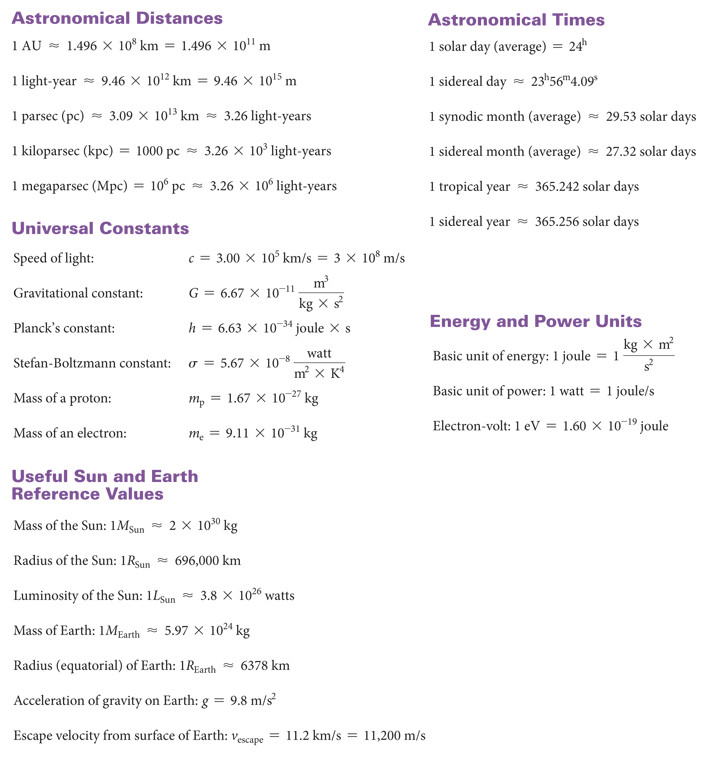
\includegraphics[scale=0.7]{constants}


\section{Lecture Slides}
\input{slides/scale.tex}
\input{slides/discovery.tex}
\input{slides/science.tex}
\input{slides/making_sense.tex}
\input{slides/light.tex}
\input{slides/telescopes.tex}
\input{slides/system.tex}
\input{slides/distant.tex}
\input{slides/life.tex}
\section{Chapter S3: Space and Time}

\subsection{Special Relativity}

Einstein's Theories of Relativity:
\begin{itemize}
\item Special Relativity: usual ideas of space and time change as we approach the speed of light ($E = mc^2$)
\begin{itemize}
\item no object can travel faster than light
\item observing a object near the speed of light:
\begin{itemize}
\item time slows down
\item length contracts in direction of motion
\item mass increases
\end{itemize}
\item simultaneousness changes based on your frame of reference
\end{itemize}
\end{itemize}

Postulates of special relativity:
\begin{itemize}
\item laws of nature are the same for everyone
\item speed of light is the same for everyone
\end{itemize}

Time Dilation: \[ t_1 = t_0\sqrt{1-\bigg(\frac{v^2}{c^2}\bigg)} \]
Length Contraction: \[ l_1 = l_0\sqrt{1-\bigg(\frac{v^2}{c^2}\bigg)} \]
Mass Increase: \[ m_1 = \frac{m_0}{\sqrt{1-\bigg(\frac{v^2}{c^2}\bigg)}} \]

Since no information can be transfered faster than the speed of light objects traveling near the speed of light will perceived information at different rates since the information is moving much more slowly relative to their speed.

\subsubsection{Tests for Relativity}
Michelson-Morley experiment found evidence for the absoluteness of the speed of light in 18887.

Time dilation occurs often to subatomic particles in accelerators.

Time dilation discovered with airplanes and very precise clocks.

$E = mc^2$ verified by measurements taken of the sun.

If the speed of light were not absolute light coming from a car moving towards you would travel at 100km/hr + c and a car moving parallel to you would be see at 100 km/hr so witnessing their collision would look very odd.

\subsection{General Relativity:}

\begin{itemize}
    \item Gravity arises from distortions of spacetime
    \item Time runs slowly in gravitational fields
    \item Rapid changes in the motion of large masses can cause \emph{gravitational waves}
\end{itemize}

\textbf{The equivalence principle:} Being on Earth (gravity = 1g) is exactly equivalent to being in space accelerating at 9.8 $m/s^2$ (1g) feel the exact same.

Motion is relative. Usually how fast your perceive something is based on your velocity compared to it. The exception is light which always is seen at the same speed (called \textbf{absolute relativity})

Worldlines:
\begin{itemize}
    \item x-axis = space
    \item y-axis = time
    \item vertical line = no motion
    \item diagonal line = constant motion
\end{itemize}

What are the effects of a curved geometry for spacetime?
\begin{itemize}
    \item The shortest path between two points is a great circle
    \item Parallel lines eventually converge
    \item Angles in triangles add up to $> 180^\circ$
    \item Circumference of a circle is $< 2\pi r$
\end{itemize}

Saddle-shaped geometry
\begin{itemize}
    \item A piece of a hyperbola is the shortest distance between two points
    \item Parallel lines diverge
    \item Angles in a triangle $< 180^\circ$
    \item Circumference of a circle is $> 2\pi r$
\end{itemize}

According to the equivalence principle if you are floating freely, then your worldline is following the \textbf{straightest possible path} through spacetime.  If you feel weight, then your path is curving.


Curvature of spacetime depends on the size of the object and the mass of the object:  If we change the size of an object without changing its mass, spacetime becomes more curved near its surface (as does the strength of gravity).

In a black hole the curvature forms a ``bottomless pit'' in spacetime.  The point of no return in a black whole is the \textbf{event horizon}, where the escape velocity surpasses the speed of light.

\subsubsection{Gravity and Time}

In an accelerating spaceship, light travels more quickly from front to back than vice versa.  So we say that time is running more quickly in the front of the spaceship.  By the equivalence principle, time runs slower at lower altitudes

\subsubsection{Evidence for general relativity}

\begin{itemize}
    \item Precession of mercury
    \item Gravitational lensing: light bends around very massive objects
    \item Gravitational time dilation
    \item Gravitational waves
    \begin{itemize}
        \item movements of a massive object can produce gravitational waves
        \item we think we have observed this in the orbits of a binary neutron star system (orbit is getting smaller as energy is carried away)
    \end{itemize}
\end{itemize}

\section{Chapter S4: Building Blocks of the Universe}

Quantum ideas
\begin{itemize}
    \item Light behaves light particles (photons)
    \item Protons and neutrons are not fundamental, they are made of quarks
    \item Antimatter can annihilate matter and produce pure energy) photons, neutrinos, etc
    \item Particles can behave like waves
\end{itemize}

Classes of particles
\begin{itemize}
    \item Bosons: photons, gluons
    \item Fermions
    \begin{itemize}
        \item Leptons: electrons, neutrinos
        \item Quarks: up, down, strange, charmed, top and bottom.  Proton = u,u,d; neutron = u,d,d
    \end{itemize}
\end{itemize}

Fermions have half-integer spin (spin is a multiple of $\frac{h}{2\pi}$).  Bosons have integer spin.

Each particle has an antimatter counterpart.  When a particle collides with its antimatter counterpart, they annihilate and become pure energy (photons) in accord with $E = mc^2$

\subsection{Fundamental Forces}

Four fundamental forces
\begin{itemize}
    \item Gravity: holds large-scale structures together. Exchange particle = gravitons
    \item Electromagnetic: holds electrons in atoms. Exchange particle = photons
    \item Strong: hold nuclei together.  Exchange particle = gluons 
    \item Weak: mediates nuclear reactions. Exchange particle = weak bosons
\end{itemize}

Relative strength
\begin{itemize}
    \item Inside nucleus
    \begin{itemize}
        \item Strong force 100 times electromagnetic
        \item Weak force is $10^{-5}$ times electromagnetic
        \item Gravity is $10^-{43}$ times electromagnetic
    \end{itemize}
    \item Inside nucleus
    \begin{itemize}
        \item Strong and weak are unimportant
    \end{itemize}
\end{itemize}

\subsection{Uncertainty}

The uncertainty principle: The more we know about where a particle is located, the less we can know about its momentum, and the converse.

Electrons do not have discrete positions, we only know the probability of finding an electron at a certain spot.

Uncertainty in location * uncertainty in momentum = Planck's constant (h)\\
Uncertainty in energy * uncertainty in time = Planck's constant (h)

Exclusion principle: Two fermions of the same type cannot occupy the same quantum state at the same time.

Degeneracy pressure: Squeezing matter restricts locations of its particles, increasing their uncertainty in momentum.  Since two particles cannot be in the same quantum state (including momentum) at the same time, so there must be an effect that limits how much matter can be compressed.

``Electron degeneracy pressure'' is what supports white dwarfs against gravity.  ``Neutron degeneracy pressure'' is what supports neutrons stars against gravity.

Quantum tunneling is when the effect of the uncertainty of subatomic particles allows them to ``tunnel'' through barriers.  This is how protons can fuse, they tunnel through the electromagnetic energy barrier.


Virtual pairs are matter-antimatter pairs of particles that rapidly appear and disappear.  The combined energy of these pairs is called the \textbf{vacuum energy}.  Particles can be produced near black holes if one member of a virtual pair falls into the black hole.  Energy to permanently create the other particle comes out of the black hole's mass --- the black hole slowly evaporates.

\input{slides/stars.tex}

\end{document}
